\chapter{Background}
\label{ch:preliminaries}

In this chapter, we outline the relevant terminologies and the theoretical  preliminaries that is essential for better understanding of this essay.
This chapter is sectioned into 3 parts.
Section \ref{sec:bck_rdf_model} describes essential concepts of RDF as a modeling language and its main serialization formats. 
In Section \ref{sec:bck_parser}, parsing techniques and methods to detect and recover syntax errors are discussed. Finally, Section \ref{sec:bck_ANTLR} presents an overview of ANTLR parser generator which is used to automatically generate the internal parser of RDF-Doctor.


\section{RDF Model}
\label{sec:bck_rdf_model}

The "Semantic Web" \cite{W3C:SemanticWebTerm:Online} term  has appeared during the transformation process of web development from "Web of documents" to "Web of data", similar to those data found in databases. 
W3C defines it as "the Web of linked data". {Figure \ref{Fig:semanticWebStack}} describes the Semantic Web Stack, proposed by W3C. It can be seen that it contains several technologies to enable the users of creating their own data stores on web, building vocabularies, and enforcing processing rules on such data.   

Subsequently, in order to make data more and more machine-readable and interchangeable between various applications, RDF model \cite{W3C:RDF-Primer:Online} has been proposed.  To elaborate, RDF model plays a fundamental role of data exchange in the layered Semantic Web Stack and links the high-level semantic web tools with low-level ones, as exhibited in {Figure \ref{Fig:semanticWebStack}}. 
	\begin{figure}[ht]
	\begin{center}
	\setlength\belowcaptionskip{-7mm}
		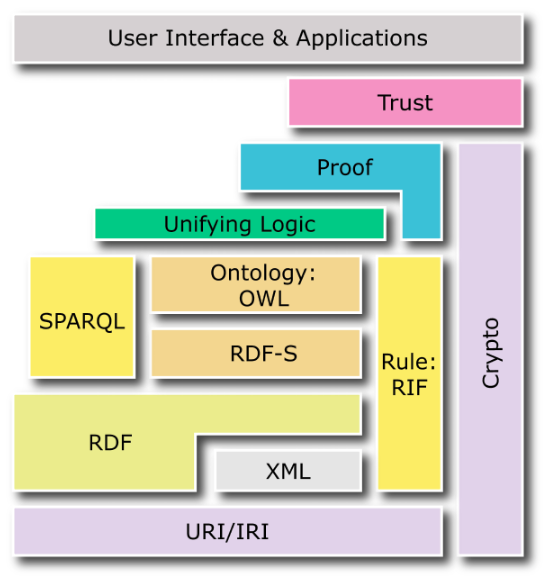
\includegraphics[scale=0.5,angle=0]{images/semanticWebStack}
		\caption{\textbf{The Semantic Web Stack \cite{W3C:SemanticStack:Online}.} RDF Model links  high-level semantic web tools with low-level ones and works as a bridge to enable data exchange between various applications}
		\label{Fig:semanticWebStack}
	\end{center}
\end{figure}
\par
Also, {Figure \ref{Fig:rdfModel}}(a) presents how data are engineered in RDF Model in triples. A triple is defined by 3 main components: a subject, a predicate, and an object. It has a common similarity of a basic structure of a simple sentence in a natural language which consists of a subject, a verb, and  an object. As the verb in natural languages shows a relation and a connection between the other two entities, in the same way in RDF Model, the predicate connects both subject and object in a certain property. 

\subsection{Simple Example of RDF Model}

To make it more clear, a simple example of RDF Modeling is giving in Figure \ref{Fig:rdfModel}(b). A fact to express that "German has the river Rhein", \textbf{Ex:Germany} is a subject, \textbf{Ex:hasRiver} is a predicate, and \textbf{"Rhein"} is an object. The first two terms are Uniform Resource Identifiers (URIs) where \textbf{Ex:} is a declared prefix label in RDF file to refer to an URI path and the following part \textbf{Germany} is an extension of the path. The last value \textbf{"Rhein"} is a literal or a string. What is given is a simple example of RDF Model to show its fundamental structure, but, in the meanwhile, more examples can be viewed at \cite{W3C:RDF-Primer:Online}.

\begin{figure}[ht]
	\begin{center}
		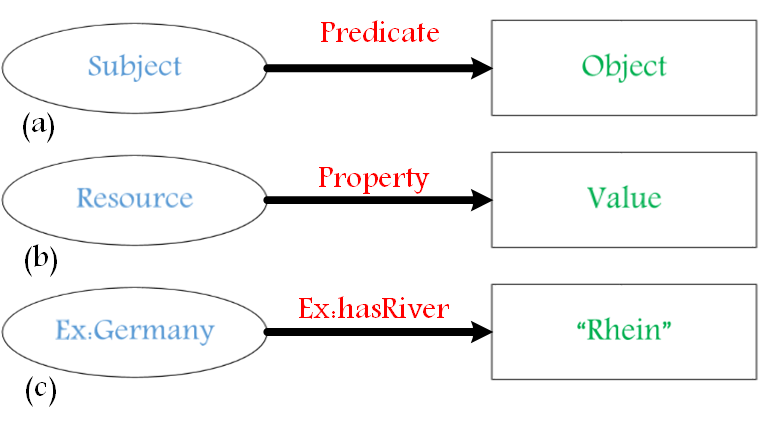
\includegraphics[scale=0.4,angle=0]{images/RDF-Model}
		\caption{\textbf{ RDF Model Structure.} A triple is a major component in RDF Model which has a form of Subject-Predicate-Object, as shown by (a), while an example of a triple is presented by (b) }
		\label{Fig:rdfModel}
	\end{center}
\end{figure}

\section{Parsing and Error Recovery}
\label{sec:bck_parser}
This subsection defines "Parsing" and "Grammar" terms, shows the role of the parser in the compiler, discusses types of parser developments, and finally, it lists the methodologies of error recovery in parsers. 
\subsection{Parsing and Grammar Definitions}
It is of great benefit to shed a light on parsing term to understand later the approach of this study. In \cite{parsingGuide2017}, Gabriele Tomassetti has defined \textbf{Parsing} by:{\it  \textbf{``The analysis of an input to organize the data according to the rule of a grammar''}}. It can be intelligibly recognized that parsing deals with some input data and tries to analyses it based on a given grammar. let's have a look on the definition of grammar based on  \cite{parsingGuide2017},as well. \textbf{Grammar} is 
{\it \textbf{``A formal grammar is a set of rules that describes syntactically a language''}}. In the definition, rules are the significant part of the grammar to define a syntax of a language.  
\subsection{Parser Role in Compilers}
The parser is an essential element in  compilers. {Figure \ref{Fig:parserPosition}} draws the role of the parser in a compiler. The first phase "Lexical Analyzer" receives the input data, then produces tokens for the next phase "Parser". Parser constructs a parse tree based on its grammar rules and gets the next token till it consumes all tokens. The parse tree as an parser's output is delivered to the next phases of a compiler. If any errors are found, lexical errors can be generated by Lexical Analyzer and Parser is the producer of both Syntax and semantic errors.%TODO{we can add more declartion about symbol table}
 A symbol table is data structure entries to store some declared values in the input, such as in programming languages object and variable names. It is used by both  Lexical Analyzer and Parser as it is shown in {Figure \ref{Fig:parserPosition}}.
%TODO{add the ref or change the image}

\begin{figure}[ht]
	\begin{center}
		\setlength\belowcaptionskip{-7mm}
		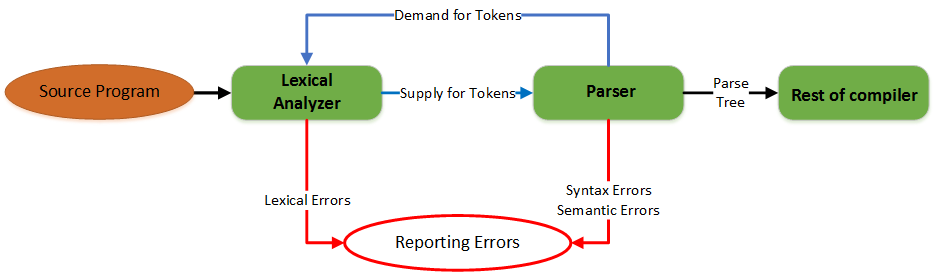
\includegraphics[scale=0.55,angle=0]{images/ParserRole}
		\caption{\textbf{Role of Parser in compilers}. a parsing part in a compiler has 2 main elements: a Lexical analyzer and a parser, the former supplies tokens to the latter, once it has enough tokens to be parsed, it parse them, and asks the former to continue of the tokens supplement, the former generates lexical errors and the latter produces syntax ans semantic errors when parsing a source program, the parse tree is the output of the latter }
		\label{Fig:parserPosition}
	\end{center}
\end{figure}
\subsection{Parser Developments}
In order to build a parser, there are two options to get such objective, either by building your own hand-written parser or getting an off-the-shelf parser generator tool. follows both approaches are discussed:
\par \textbf{1) Hand-writing Parsers:} someone writes his own parser, including the lexical analyzer and the parser. On the one hand this way gives more flexibility in handling several problems triggered during development but on the other hand it consumes much time and mind.
\par \textbf{2) Parser Generators:} someone uses a tool to generate a parser to do specific parsing task, by writing a compatible grammar to such tool. The most advantage of using those tools is the less consumed time to build a parser.  

\subsection{Error Recovery Methodologies in Parsers}
Error Recovery Strategies are the behavior of a system once an error is detected. Compiler's researchers Aho et al \cite{Aho:2006}  have classified such methodologies as follows:
\begin{itemize}
	\item \textbf{Panic-Mode Recovery}: once an error has been discovered, the parser ignores and skips next input symbols one by one till a recognized set of tokens is detected. In spite of discarding sometimes huge amount of input symbols with checking them for further error detection, it is considered a simple parsing mode and do not fall in an infinite loop while other modes may do.
	\item \textbf{Phrase-Level Recovery}: to continue the parsing process, the parser performs local correction. A typical local correction in RDF is to insert a missing dot or delete extraneous dots.
	\item \textbf{Error Productions}: by expecting the common errors, production rules can be inserted into the grammar. Then, the generated parser is well-informed about such errors. Error diagnostics can be easily done in this case since the error in our hand.
	\item \textbf{Global Correction}: the parser tries to reduce as much as possible number of change operations (Insertion, deletion or modification) when dealing with an incorrect input token to reduce globally total cost of error correction. To make it more clear, let's assume an incorrect input statement X is giving in grammar G, the parser constructs a closest error-free parse tree of statement Y to replace statement X, such that changes are small as possible. 
\end{itemize}


\section{ANTLR Parser Generator}
\label{sec:bck_ANTLR}

ANTLR is an handy tool and easy way to generate a specific domain language parser. It is an parser generator to do automatic generation of a source code of such parser without much coding and with less time. The basic principle used by ANTLR is define language's rules which draws the syntax and the semantic of the language the parser build for. 
\par
 As has been previously discussed, the compiler has two main subsystems: lexer and parser. Both lexer and parser are needed to have their rules defined in ANTLR grammar file.  {Figure \ref{Fig:ANTLR}} demonstrates an auto-generated parser program, generated based on ANTLR tool. follows is a sequence steps \citealp{ANTLR:Tool:Online}, describes such parsing process:

\begin{figure}[ht]
	\begin{center}
		\setlength\belowcaptionskip{-7mm}
		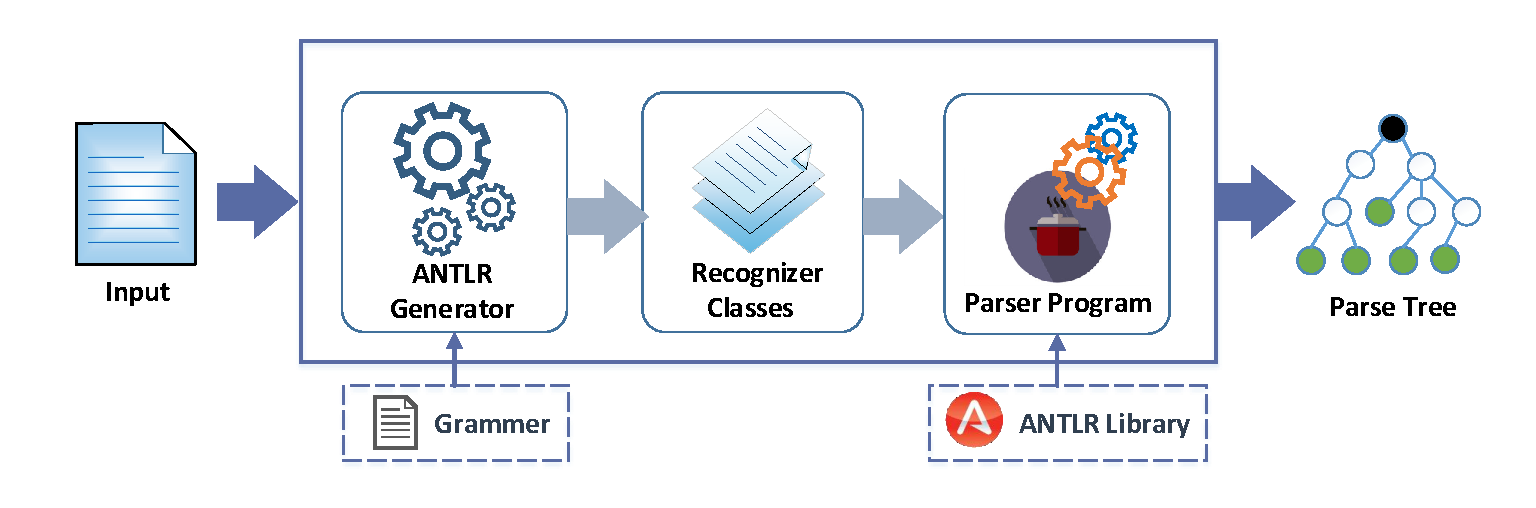
\includegraphics[scale=0.6]{images/ANTLR}
		\caption{\textbf{Parsing process based on ANTLR parser generator.} ANTLR parser generator receives the grammar file to generate the classes of the lexer and the parser, when the input text is submitted, the generated classes with using of ANTLR library start the parsing process to generate the parse tree}
		\label{Fig:ANTLR}
	\end{center}
\end{figure}


\begin{enumerate}
		
		\item  {\bf Writing a grammar file:} ordinarily, a grammar called a parsing expression grammar, or PEG is required to build a parser. ANTLR needs a context-free grammar, crafted with Extended Backus-Naur Form (EBNF). EBNF consists of a sequence of rules. These rules describe the syntax and the semantic of an input which needs to be parsed. Either Terminal or Non-terminal entities are the components of these rules. On the one hand, Terminals are the leaf elements where they have no grammatical structure, e.g., words or numbers. On the other hand, Terminal entities are those with a definite grammatical structure and name, e.g., triple component. 
		\item {\bf Generation of recognizer target\_based classes by ANTLR generator:} a significant feature of ANTLR is its capability of generated the auto-generated parse code for  a variety of the programming languages \citealp{ANTLR:Website:Online}: Java, C\#, Python (2 and 3), JavaScript, Go, C++, and Swift.
		\item {\bf Feeding an input file for parsing:} as an input, ANTLR can parse text documents without additional libraries. Users send their input files for parsing where the parsing process will be achieved based on the crafted grammar in the first step.
		\item {\bf Parsing procedure:} {Figure \ref{Fig:ANTLR} } shows that it is the cooking time in this step where all materials and Ingredients are ready. The materials are: 1) the auto-generated parser, 2) the ANTLR library. The ingredients are one or more text files to be parsed. 
		\item {\bf Delivering of a report and parse tree as an output:} now the cake is ready for eating, an output of this process is given. A parse tree and a report of collected errors can be such output.
	\end{enumerate}











